\documentclass[11pt]{article}

\usepackage[utf8]{inputenc}
\usepackage{float}
\usepackage[colorlinks,citecolor=blue,urlcolor=blue]{hyperref}
\usepackage[pdftex]{graphicx}
\usepackage{parskip}
\usepackage{subfig}
\usepackage{fullpage}
\usepackage{amsmath}
\usepackage{amssymb}
\usepackage{color}
\usepackage{todonotes}
\usepackage{listings}
\usepackage{common}
\usepackage{bm}
\usepackage{enumitem}
\usepackage{tikz}
\usepackage{soul}
\usepackage{framed}
\usepackage{pythonhighlight}
\usepackage{common}
\usepackage{booktabs}

\title{Supervised Machine Learning for Biomolecular Condensate Quantification and Measurement}
\author{Rodney Lafuente Mercado \\ lafuentemercado@college.harvard.edu}
\date{May 4, 2022}
\begin{document}

\maketitle{}

\begin{abstract}
\noindent This report details the background, approach, and process of applying supervised machine
learning methods for identification of biomolecular condensates in SARS-CoV-2 nuclecaspids. The
report covers not only the feature and model selection of the process but also the stuff regarding
splitting and segmenting and filtering as well.
\end{abstract}

\section{Background}

The motivation behind this project is to quantify the effect of different compounds on condensate
formation in SARS-CoV-2 nucleocaspids. This is part of a larger study in what things affect what in
what. Current methods such as software like MetaXpress are effective but there is suspicion that
machine learning may be way better at the identification. The method outlined in this paper is
inspired by Ilatisk, albeit with different methods to handle false positives. Images analyzed in
this project were of these nucleocaspids under three different wavelengths. These three wavelengths
are visualized in Figure~\ref{fig:wavelengths} for an example image (KRD-211028-p5\_G24\_s4).

\begin{figure}[H]
    \centering
    {
        \subfloat[Wavelength 1]{
            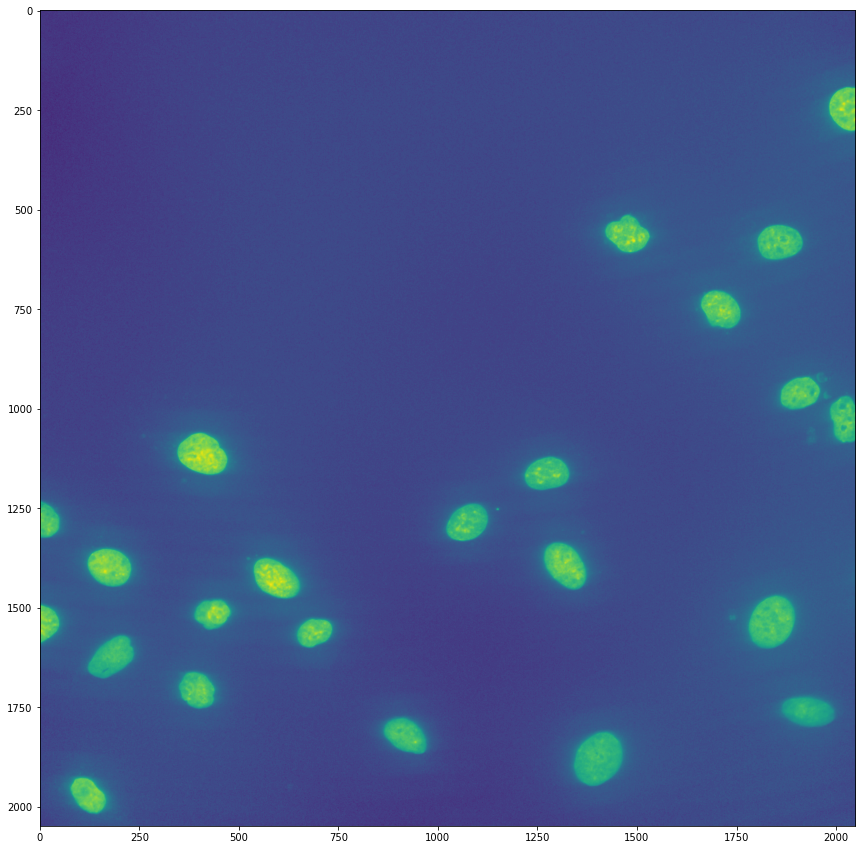
\includegraphics[width=0.3\textwidth]{wavelength_1.png}
        }
        \subfloat[Wavelength 2]{
            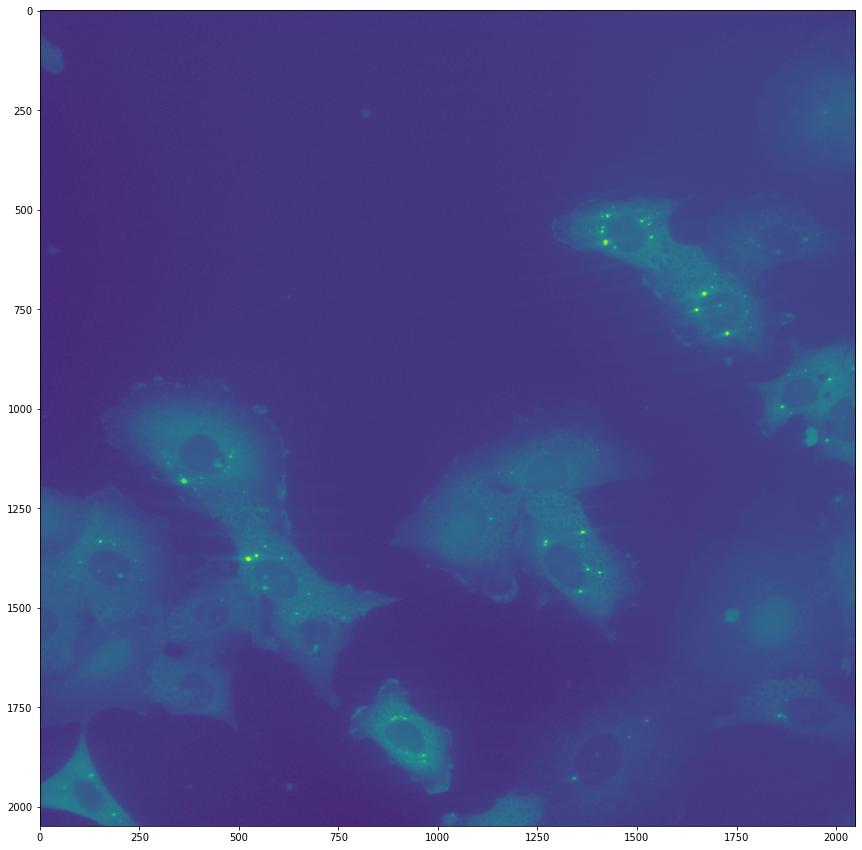
\includegraphics[width=0.3\textwidth]{wavelength_2.png}
        }
        \subfloat[Wavelength 3]{
            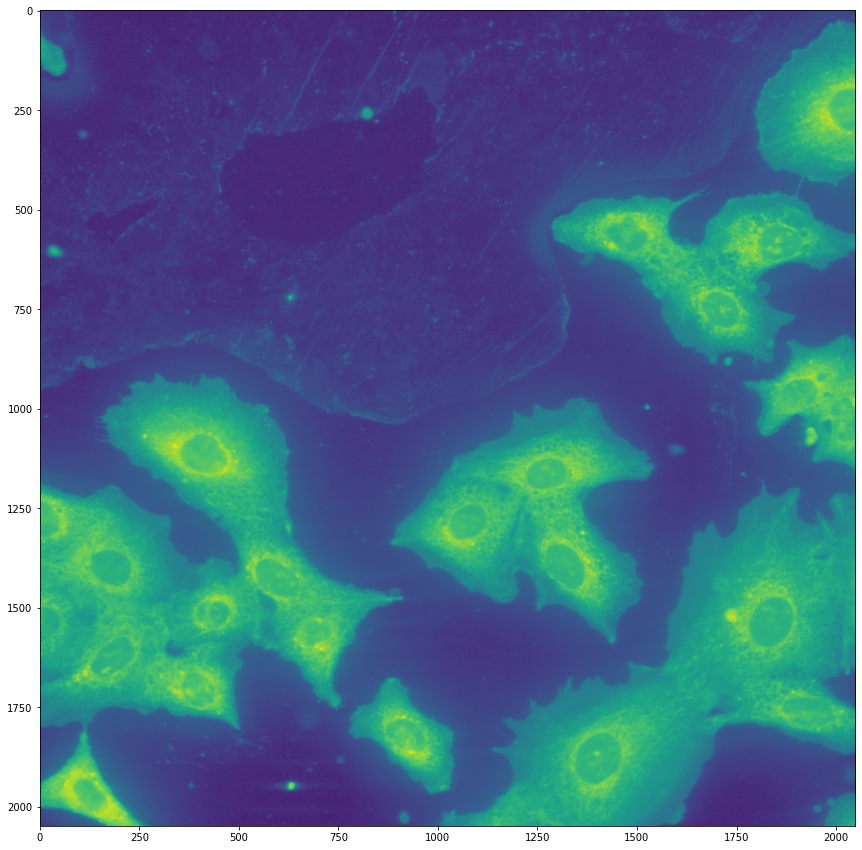
\includegraphics[width=0.3\textwidth]{wavelength_3.png}
        }
    }\caption{Example of Well Site Wavelengths}
    \label{fig:wavelengths}
\end{figure}

\noindent the wavelengths displayed each play a different purpose as is illustrated below. This
report will split the process into three sections, namely the approach to cell segmentation, feature
selection, and model selection. 


\section{Cell Segmentation}

Machine learning methods in the approach outlined in this report work only to classify pixels as
belonging to a biomolecular condensate or not. An additional component in the process of identifying
and measuring condensates is to identify areas of interest in an image, namely, differing regions
that belong to cells. Once these regions of interest are identified, condensates located in these
regions, and only in these regions, can be quantified.

\subsection{Approach}

Cell segmentation was accomplished using watershed segmentation, an algorithm that takes as input
binary images that it treats as topological maps such that they are flooded in order to find the
proper separation between regions. This method, as well as all other methods outlined in this
report, are implemented using the ScikitImage and ScikitLearn Python libraries. For identifying
separate regions, a mask identifying nuclei was used. For identifying regions containing cytoplasm,
a mask identifying cytoplasm was used. 

The masking process, an example of which can be seen below, involves the computation of a certain
threshold that must be high enough such that only pixels of a desirable intensity are retained. The
method for nuclei mask creation was to use Otsu's method of thresholding. This method aims to
minimize the variance between . The two thresholding methods were chosen by applying a variety of
different thresholding mechanisms to the images and picking the ones best differentiating between
cells in the end. 

\subsection{Results}

Figure~\ref{fig:masking_process} displays the full masking process, save for a step that removes
cells from the mask that overlap with the an outlier mask. This step is visualized using a different
example image in Figure~\ref{fig:outlier_removal}.

\begin{figure}[H]
    \centering
    {
        \subfloat[Wavelength 1]{
            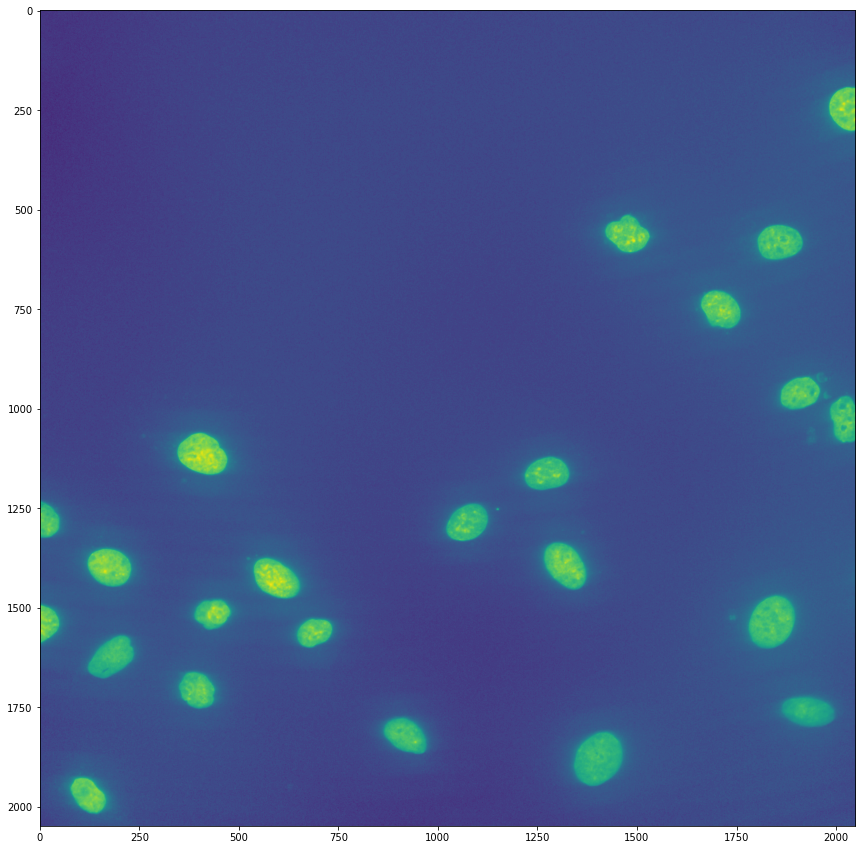
\includegraphics[width=0.3\textwidth]{wavelength_1.png}
        }
        \subfloat[Nuclei Mask]{
            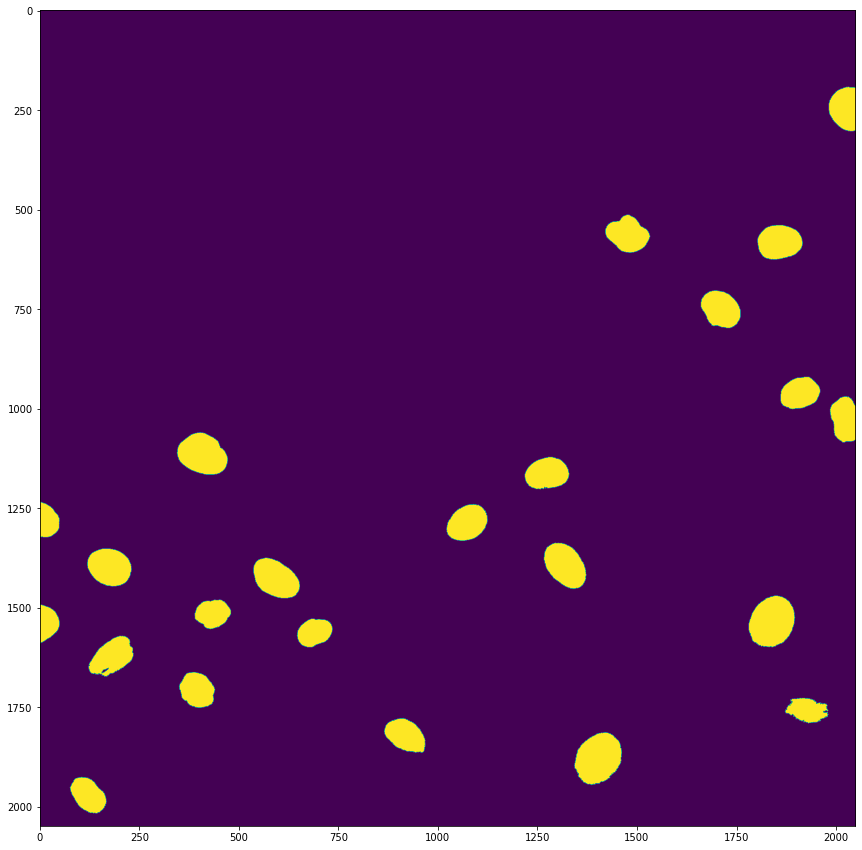
\includegraphics[width=0.3\textwidth]{nuclei_mask.png}
        }
    }\hfill{
        \subfloat[Wavelength 3]{
            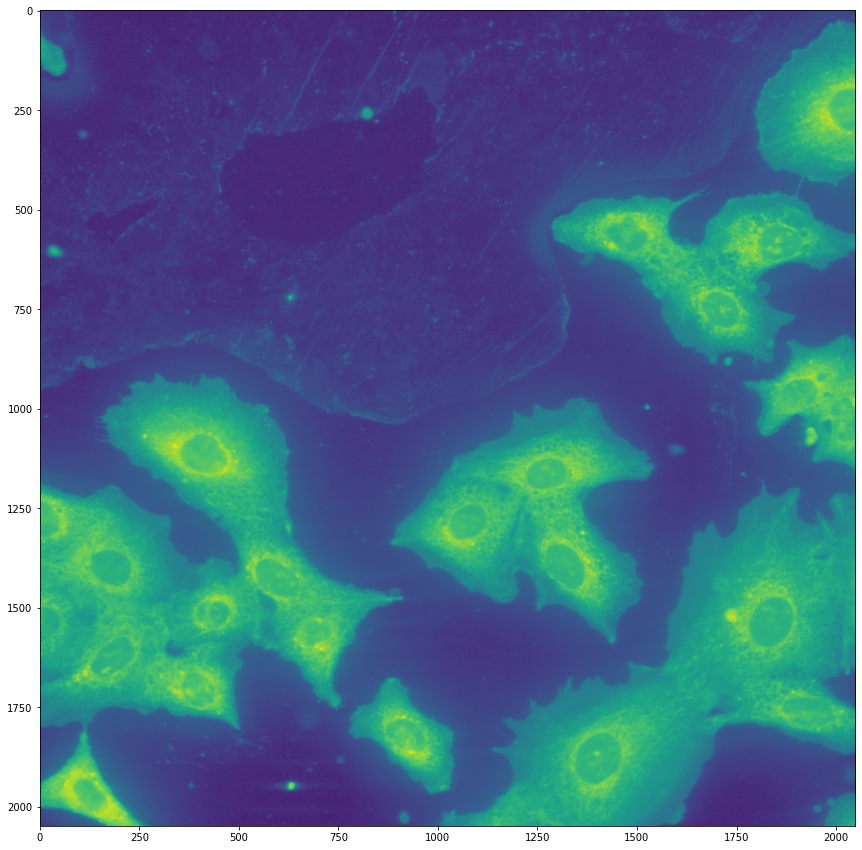
\includegraphics[width=0.3\textwidth]{wavelength_3.png}
        }
        \subfloat[Cytoplasm Mask]{
            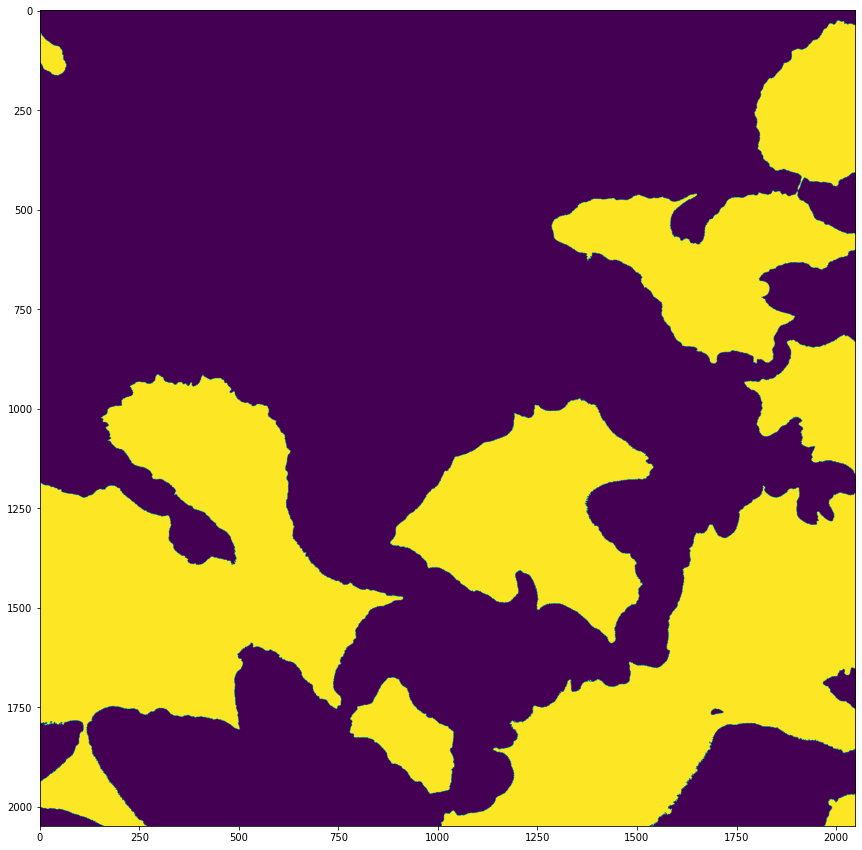
\includegraphics[width=0.3\textwidth]{cytoplasm_mask.png}
        }
    }\hfill{
        \subfloat[Segmented Cells (Nuclei for clarity)]{
            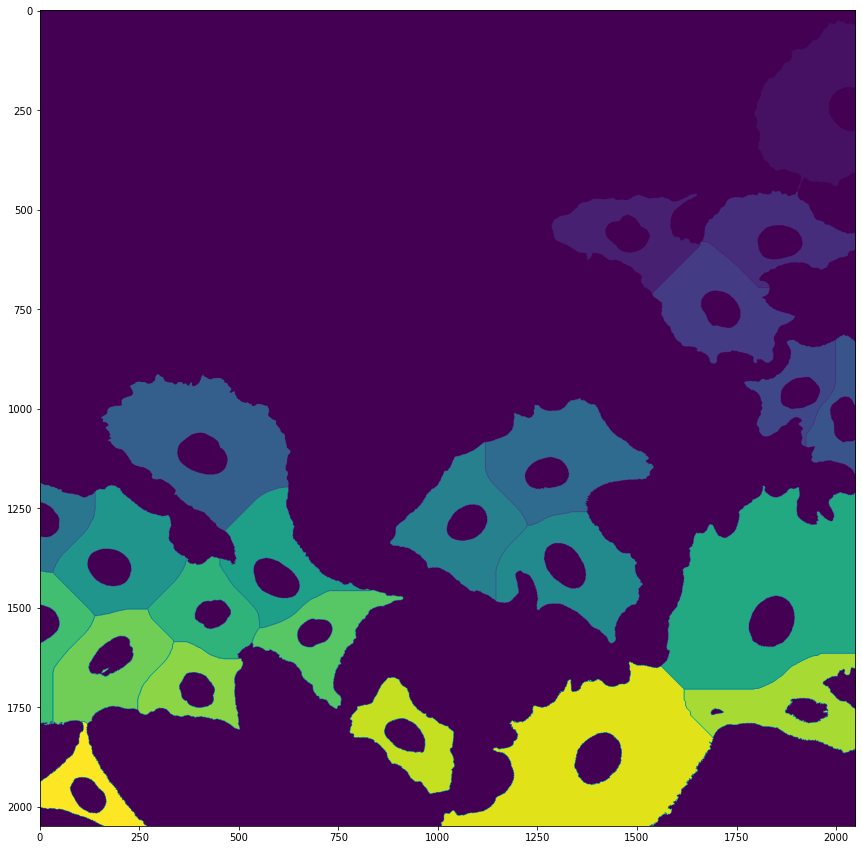
\includegraphics[width=0.3\textwidth]{combined_mask.png}
        }
        \subfloat[Resulting Mask (Border and Outlier Cells Removed)]{
            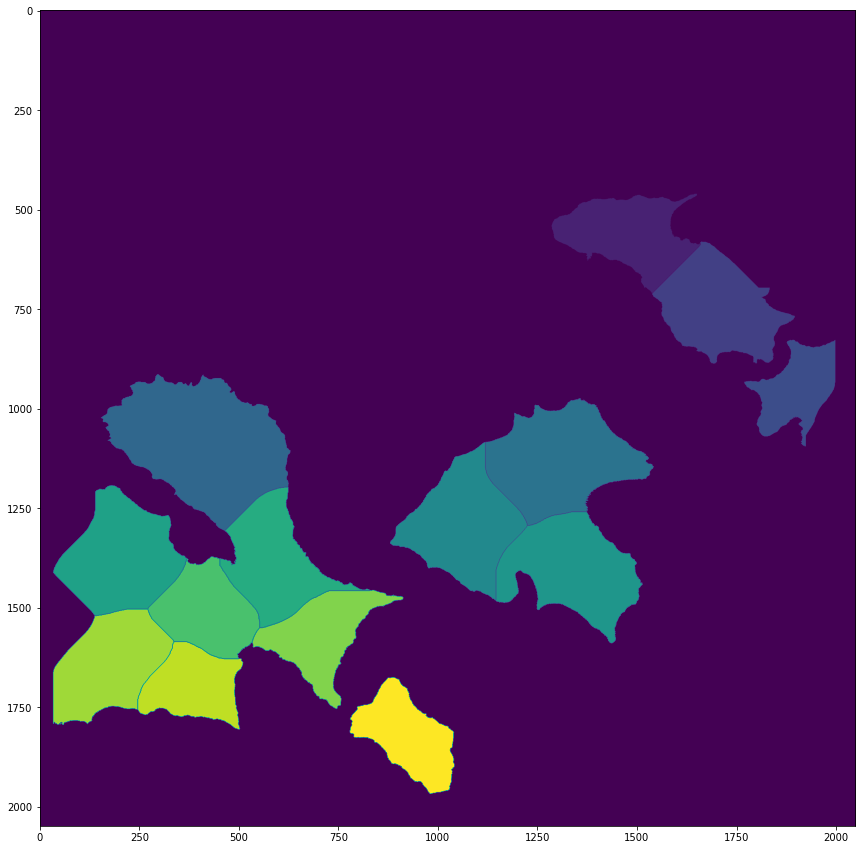
\includegraphics[width=0.3\textwidth]{final_mask.png}
        }
    }\caption{Full Masking Process}
    \label{fig:masking_process}
\end{figure}

\begin{figure}[H]
    \centering
    {
        \subfloat[Wavelength 1]{
            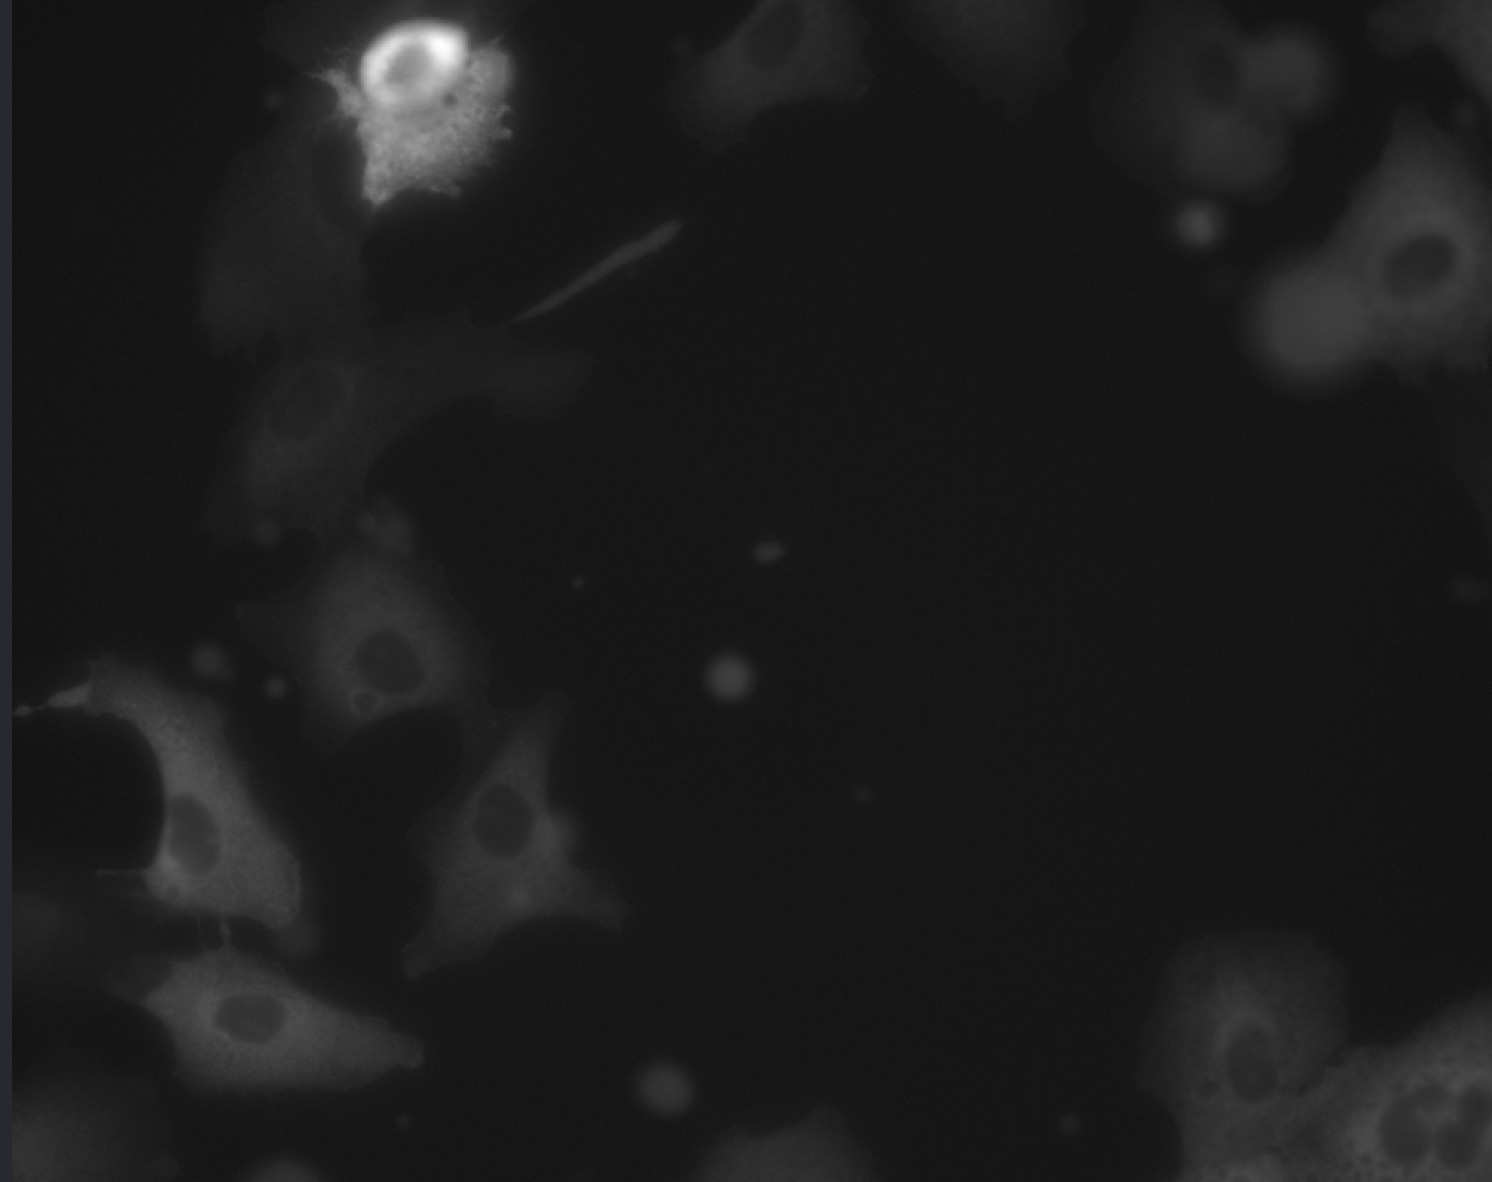
\includegraphics[width=0.5\textwidth]{bright_spot.png}
        }
    }
    {
        \subfloat[Wavelength 3]{
            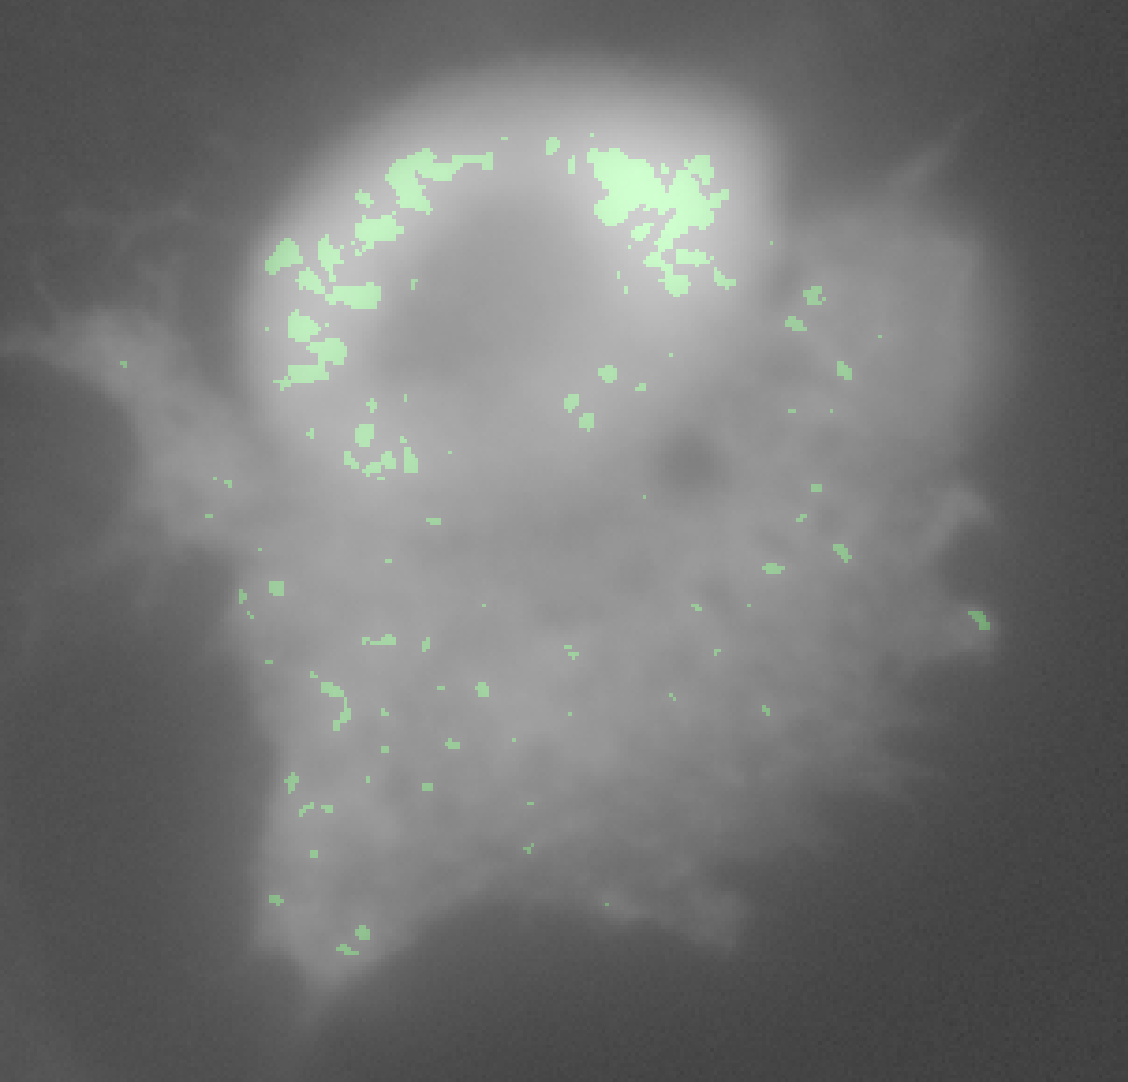
\includegraphics[width=0.5\textwidth]{bright_spot_labels.png}
        }
    }\caption{Bright Spot and Effect}
    \label{fig:bright_spot}
\end{figure}


\begin{figure}[H]
    \centering
    {
        \subfloat[Wavelength 1]{
            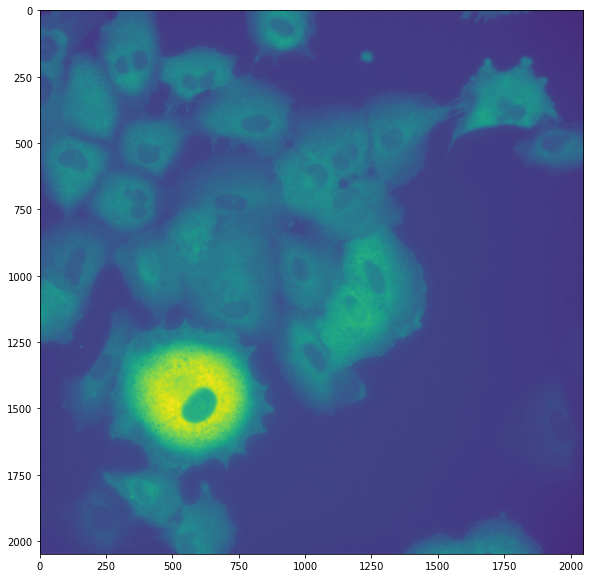
\includegraphics[width=0.3\textwidth]{bright_wellsite.png}
        }
        \subfloat[Nuclei Mask]{
            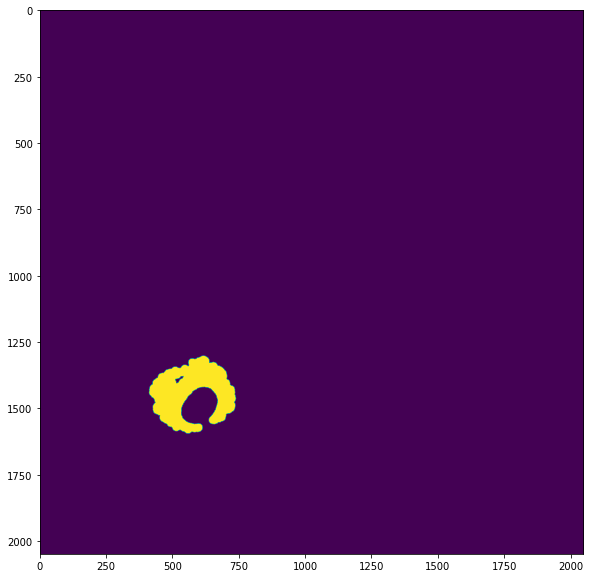
\includegraphics[width=0.3\textwidth]{bright_wellsite_outlier.png}
        }
    }\hfill{
        \subfloat[Wavelength 3]{
            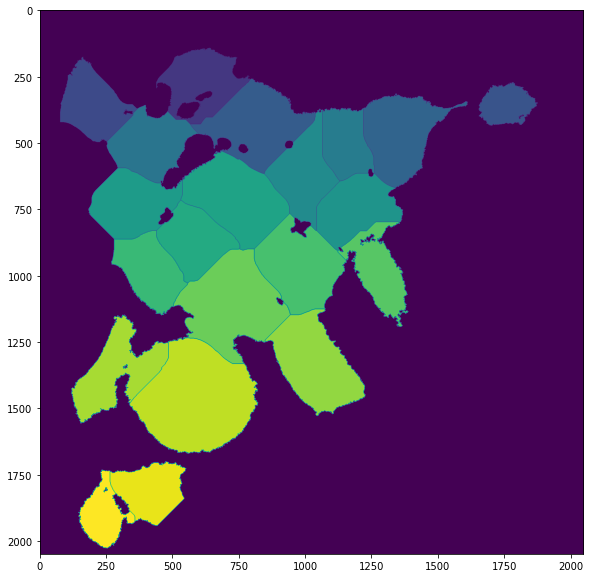
\includegraphics[width=0.3\textwidth]{bright_wellsite_premask.png}
        }
        \subfloat[Cytoplasm Mask]{
            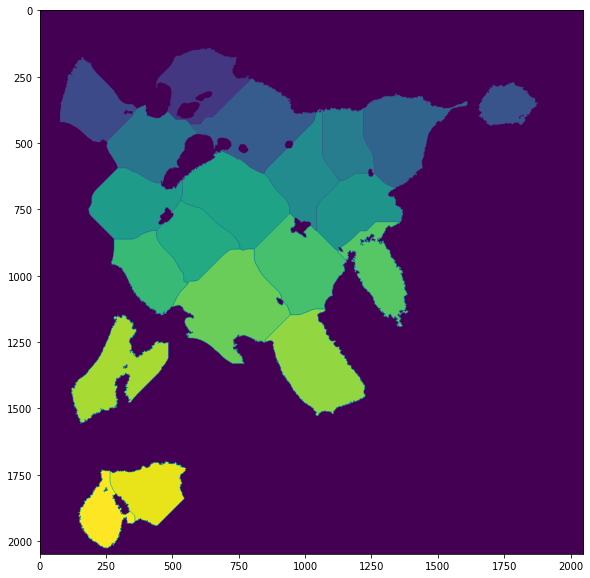
\includegraphics[width=0.3\textwidth]{bright_wellsite_mask.png}
        }
    }\caption{Outlier Removal Process}
    \label{fig:outlier_removal}
\end{figure}


This method was accurate enough to meaningfully separate condensates by which cells they belonged
to, but definitely had its drawbacks. While this method was not perfect for this perfect, it is
difficult to imagine a better method given the difficulty of segmenting cells by hand; boundaries
between cells are, more often than not, not clear in the images in which they are presented. 

\section{Feature Selection}
Classification of pixels into condensate and non-condensate regions requires not only a labeled data
set of pixels but also a way of determining which properties of those pixels are to be used for
classification purposes. For this model, we ran two different types of features: Gaussian Blurring,
for determining intensity at the pixel and in areas surrounding the pixel, as well as eigenvalues of
the Hessian matrix 

\subsection{Approach}

Supervised machine learning requires not only a labeled data set but also a method of extrapolating
information on that data prior to discerning between different classes for each of the data points. 

\subsection{Results}

Figure~\ref{fig:gaussian_blurring} shows the outcome of applying several blurring filters to an 
example well site.

\begin{figure}[H]
    \centering
    {
        {
            \subfloat[Regular Image]{
                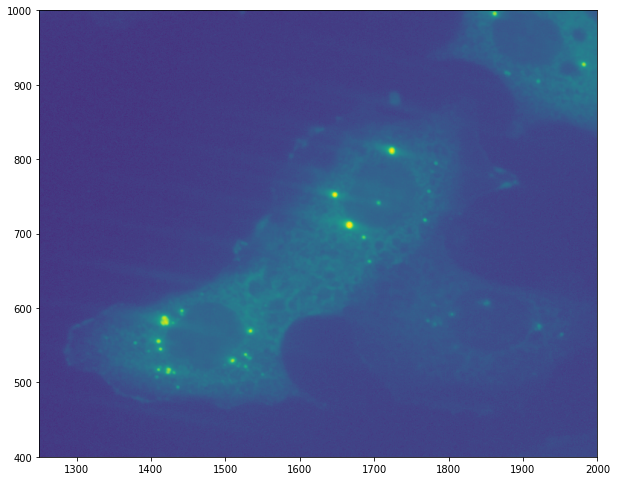
\includegraphics[width=0.3\textwidth]{zoomed.png}
            }
        }\hfill{
            \subfloat[$\sigma=1$]{
                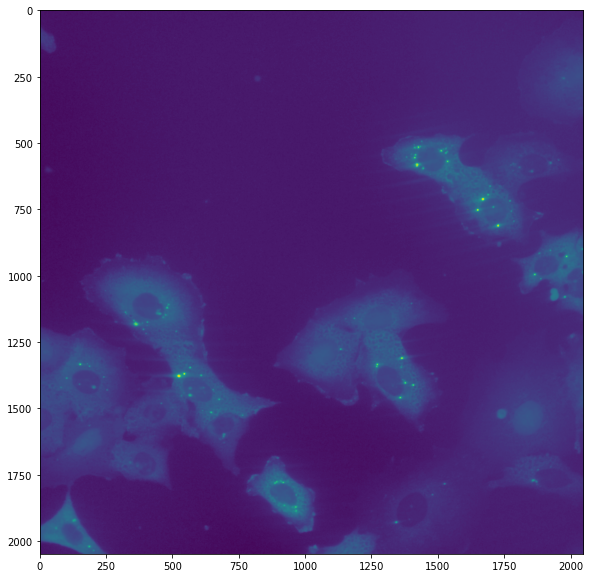
\includegraphics[width=0.3\textwidth]{gauss_blur_1.png}
            }
            \subfloat[$\sigma=2$]{
                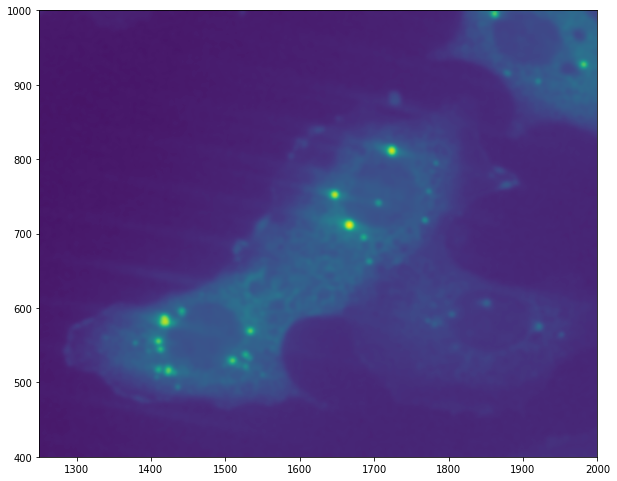
\includegraphics[width=0.3\textwidth]{gauss_blur_2.png}
            }
        }\hfill{
            \subfloat[$\sigma=4$]{
                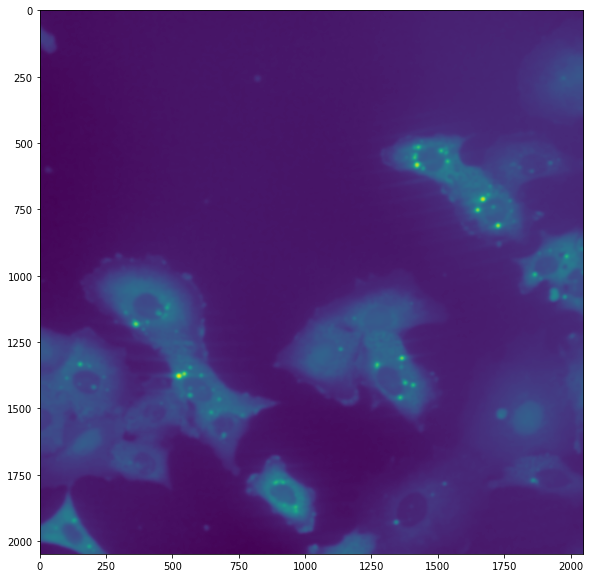
\includegraphics[width=0.3\textwidth]{gauss_blur_4.png}
            }
            \subfloat[$\sigma=8$]{
                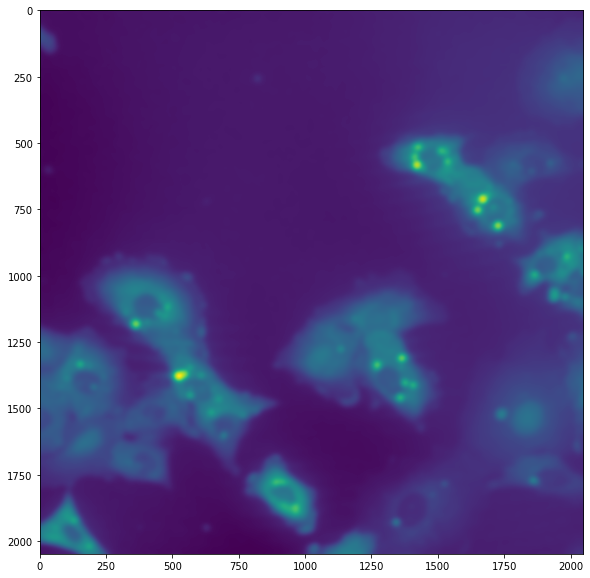
\includegraphics[width=0.3\textwidth]{gauss_blur_8.png}
            }
        }
    }\caption{Gaussian Blurring Filters}
    \label{fig:gaussian_blurring}
\end{figure}

Figure~\ref{fig:hessian} shows the outcome of extracting the hessian filters from an 
example well site.

\begin{figure}[H]
    \centering
    {
        {
            \subfloat[Regular Image]{
                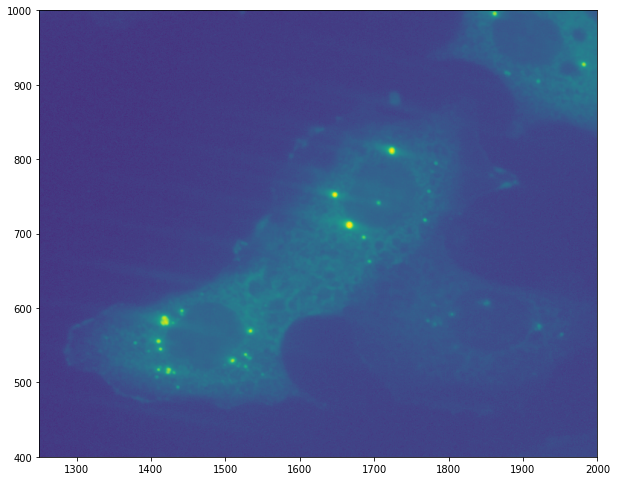
\includegraphics[width=0.3\textwidth]{zoomed.png}
            }
        }\hfill{
            \subfloat[$\sigma=4$, Hxx]{
                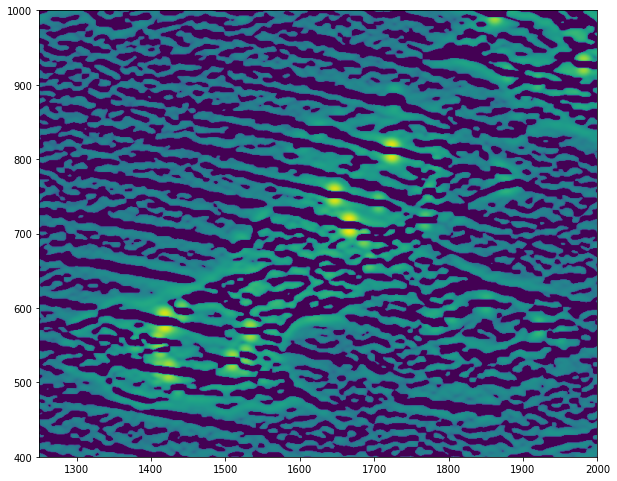
\includegraphics[width=0.3\textwidth]{zoomed_hessian_xx.png}
            }
            \subfloat[$\sigma=4$, Hxy]{
                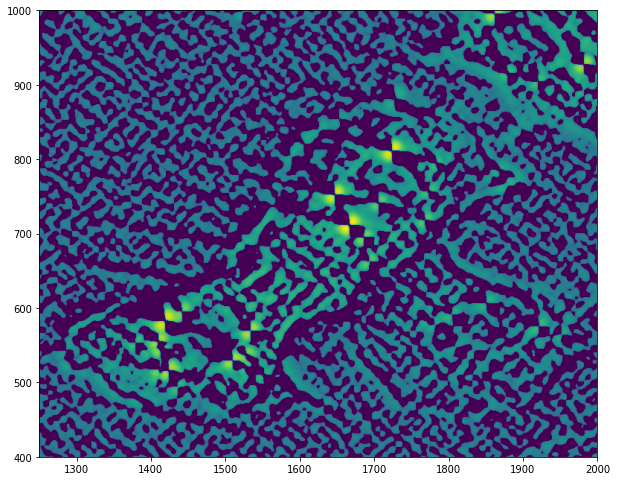
\includegraphics[width=0.3\textwidth]{zoomed_hessian_xy.png}
            }
            \subfloat[$\sigma=4$, Hyy]{
                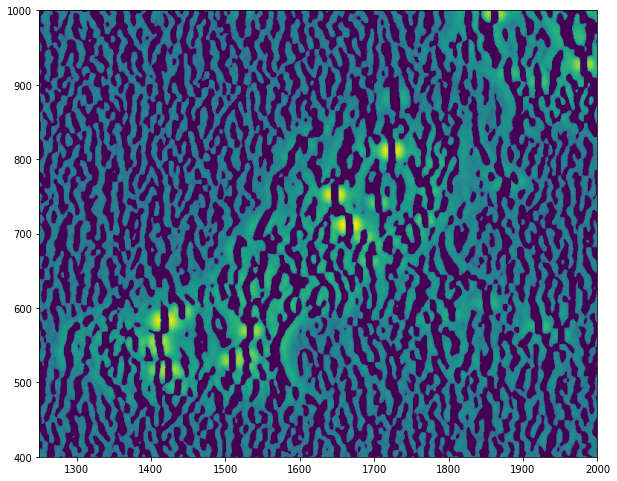
\includegraphics[width=0.3\textwidth]{zoomed_hessian_yy.png}
            }
        }\hfill{
            \subfloat[$\sigma=4$, Smaller Eigenvalues]{
                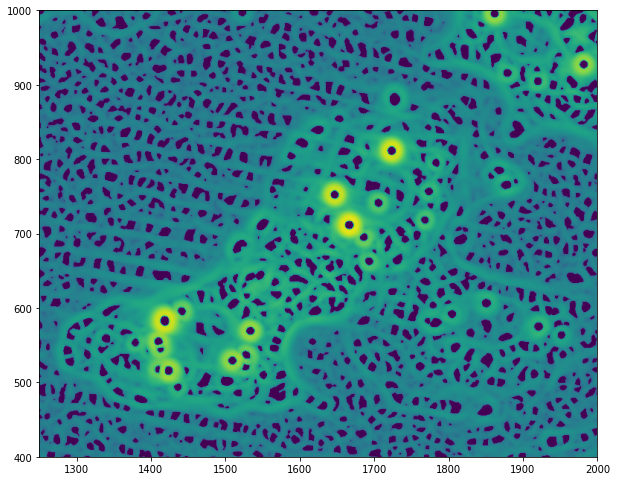
\includegraphics[width=0.3\textwidth]{zoomed_texture_4_1.png}
            }
            \subfloat[$\sigma=4$, Larger Eigenvalues]{
                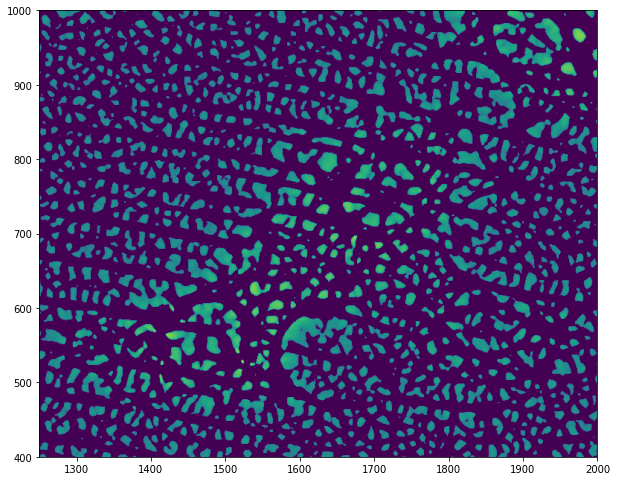
\includegraphics[width=0.3\textwidth]{zoomed_texture_4_2.png}
            }
        }
    }\caption{Gradients and Hessian Eigenvalues}
    \label{fig:hessian}
\end{figure}

Figure~\ref{fig:texture} shows the outcome of applying several texture filters to an 
example well site.

\begin{figure}[H]
    \centering
    {
        {
            \subfloat[$\sigma=1$, Smaller Eigenvalues]{
                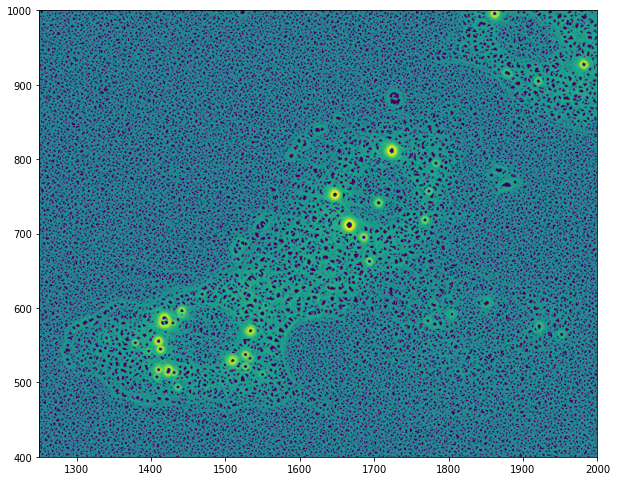
\includegraphics[width=0.3\textwidth]{zoomed_texture_1_1.png}
            }
            \subfloat[$\sigma=1$, Larger Eigenvalues]{
                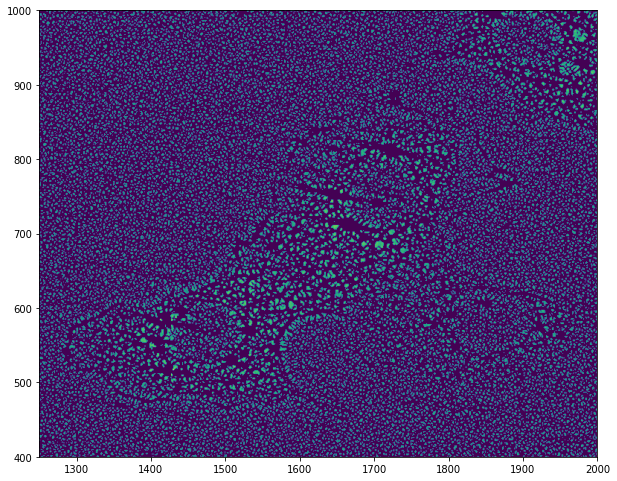
\includegraphics[width=0.3\textwidth]{zoomed_texture_1_2.png}
            }
        }\hfill{
            \subfloat[$\sigma=2$, Smaller Eigenvalues]{
                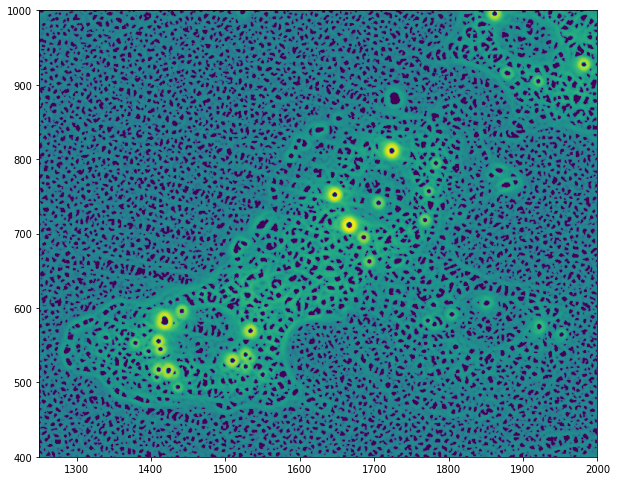
\includegraphics[width=0.3\textwidth]{zoomed_texture_2_1.png}
            }
            \subfloat[$\sigma=2$, Larger Eigenvalues]{
                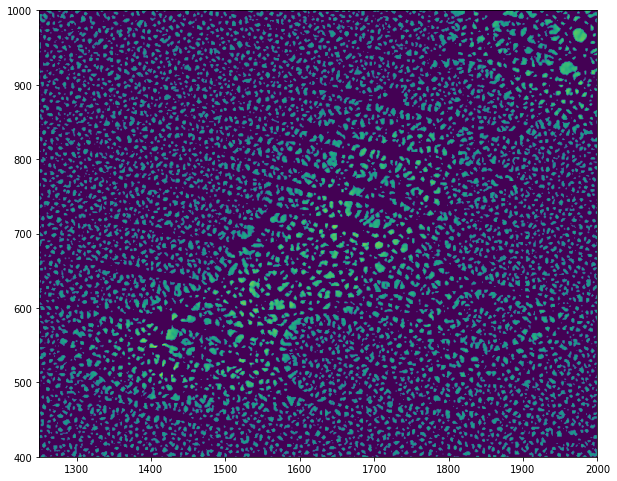
\includegraphics[width=0.3\textwidth]{zoomed_texture_2_2.png}
            }
        }\hfill{
            \subfloat[$\sigma=4$, Smaller Eigenvalues]{
                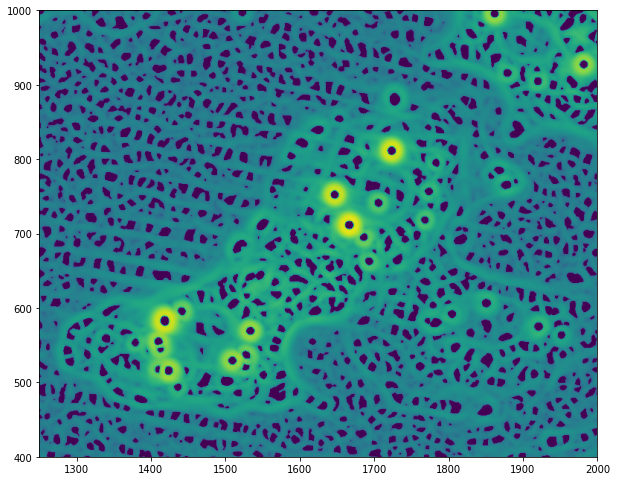
\includegraphics[width=0.3\textwidth]{zoomed_texture_4_1.png}
            }
            \subfloat[$\sigma=4$, Larger Eigenvalues]{
                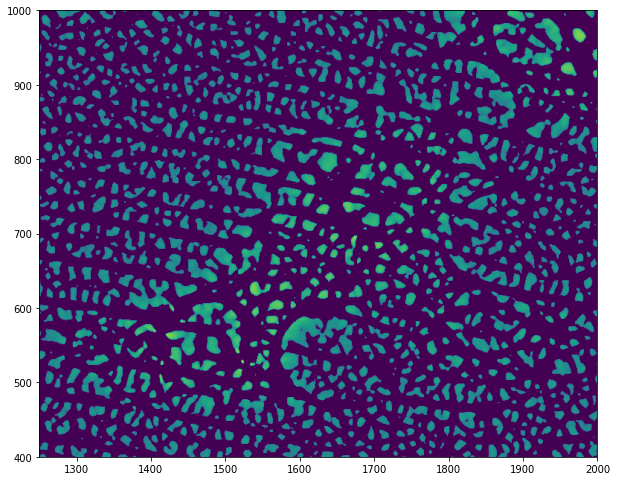
\includegraphics[width=0.3\textwidth]{zoomed_texture_4_2.png}
            }
        }\hfill{
            \subfloat[$\sigma=8$, Smaller Eigenvalues]{
                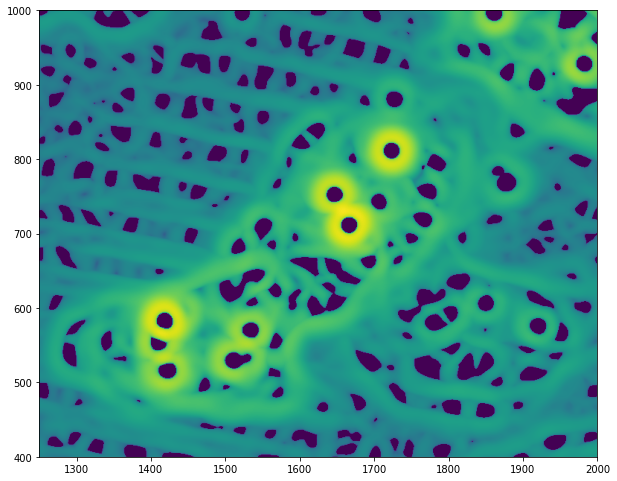
\includegraphics[width=0.3\textwidth]{zoomed_texture_8_1.png}
            }
            \subfloat[$\sigma=8$, Larger Eigenvalues]{
                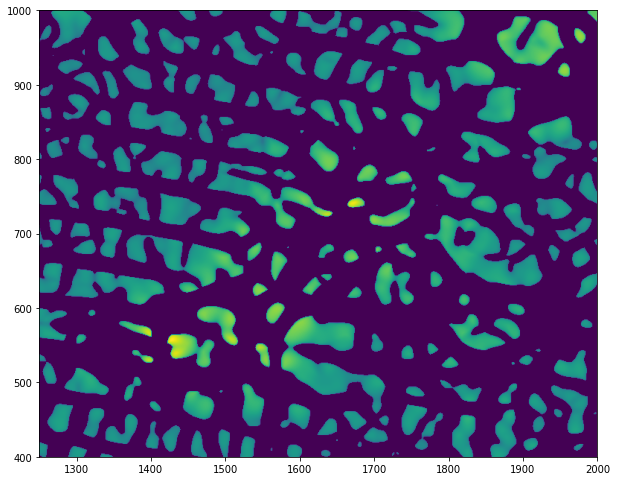
\includegraphics[width=0.3\textwidth]{zoomed_texture_8_2.png}
            }
        }
    }\caption{Full Range of Texture Filters}
    \label{fig:texture}
\end{figure}


\section{Model Selection}

Ilastik, the software that implements similar machine learning techniques for pixel classification,
uses random forest classifiers. We opted for this same model class for our dataset given that RFCs
are effective in modeling distinctions in data points from data sets of limited length.

\subsection{Approach}

What did you do? When relevant, provide mathematical descriptions or pseudocode. Credit will be
given for:

\subsection{Results}
\begin{figure}[H]
    \centering
    {
        {
            \subfloat[Drawn Labels]{
                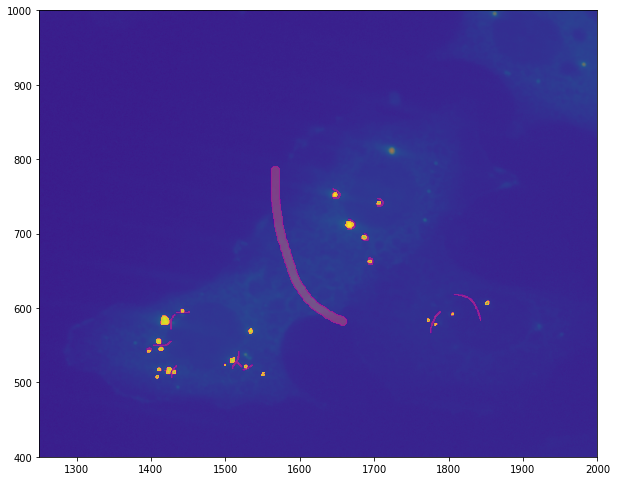
\includegraphics[width=0.5\textwidth]{y_true.png}
            }
        }
        {
            \subfloat[Prediction Result]{
                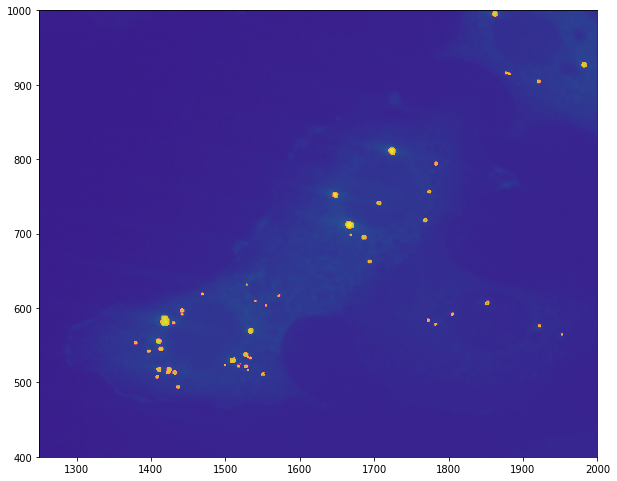
\includegraphics[width=0.5\textwidth]{y_pred.png}
            }
        }
    }\caption{True and Predicted Labels}
    \label{fig:labels}
\end{figure}

\begin{table}[H]
    \centering
    \begin{tabular}{llrrr}
        \toprule
        \# Estimators & & Intensity Features & Texture Features & Overall Rank \\
        \midrule
        \textsc{360} & & 0.9813 & 0.9811 & 5 \\
        \textsc{400} & & 0.9816 & 0.9813 & 3 \\
        \textsc{440} & & 0.9818 & 0.9814 & 4 \\
        \textsc{480} & & 0.9807 & 0.9816 & 1 \\
        \textsc{520} & & 0.9814 & 0.9811 & 1 \\
        \bottomrule
    \end{tabular}
    \caption{\label{tab:rf_search_results} Balanced Accuracies of Random Forest Models of Varying Estimator Counts}
\end{table}
    
\begin{table}[H]
    \centering
    \begin{tabular}{llrrr}
        \toprule
        C Value & & Intensity Features & Texture Features & Overall Rank \\
        \midrule
        \textsc{0.001} & & 0.8388 & 0.8839 & 5 \\
        \textsc{0.01}  & & 0.8865 & 0.9330 & 4 \\
        \textsc{0.1}   & & 0.9257 & 0.9513 & 3 \\
        \textsc{1}     & & 0.9513 & 0.9611 & 2 \\
        \textsc{10}    & & 0.9701 & 0.9677 & 1 \\
        \bottomrule
    \end{tabular}
    \caption{\label{tab:svm_search_results} Balanced Accuracies of Support Vector Machine Models of Varying C Values}
\end{table}

The results suggest that there is not much benefit to applying filters intended to identify edges
and texture like we did above. This is a surprising result, as virtually all traditional methods
(e.g., no machine learning) in image processing that are used to identify blobs and other features in
images rely on heavy filtering techniques. As for the accuracy of the results, the pixel
classification suggests that the methods are accurate in differentiating between pixels belonging to
and not belonging to condensates.

\subsection{Results}
The predictions performed as expected.

\begin{figure}[H]
    \centering
    {
        {
            {
                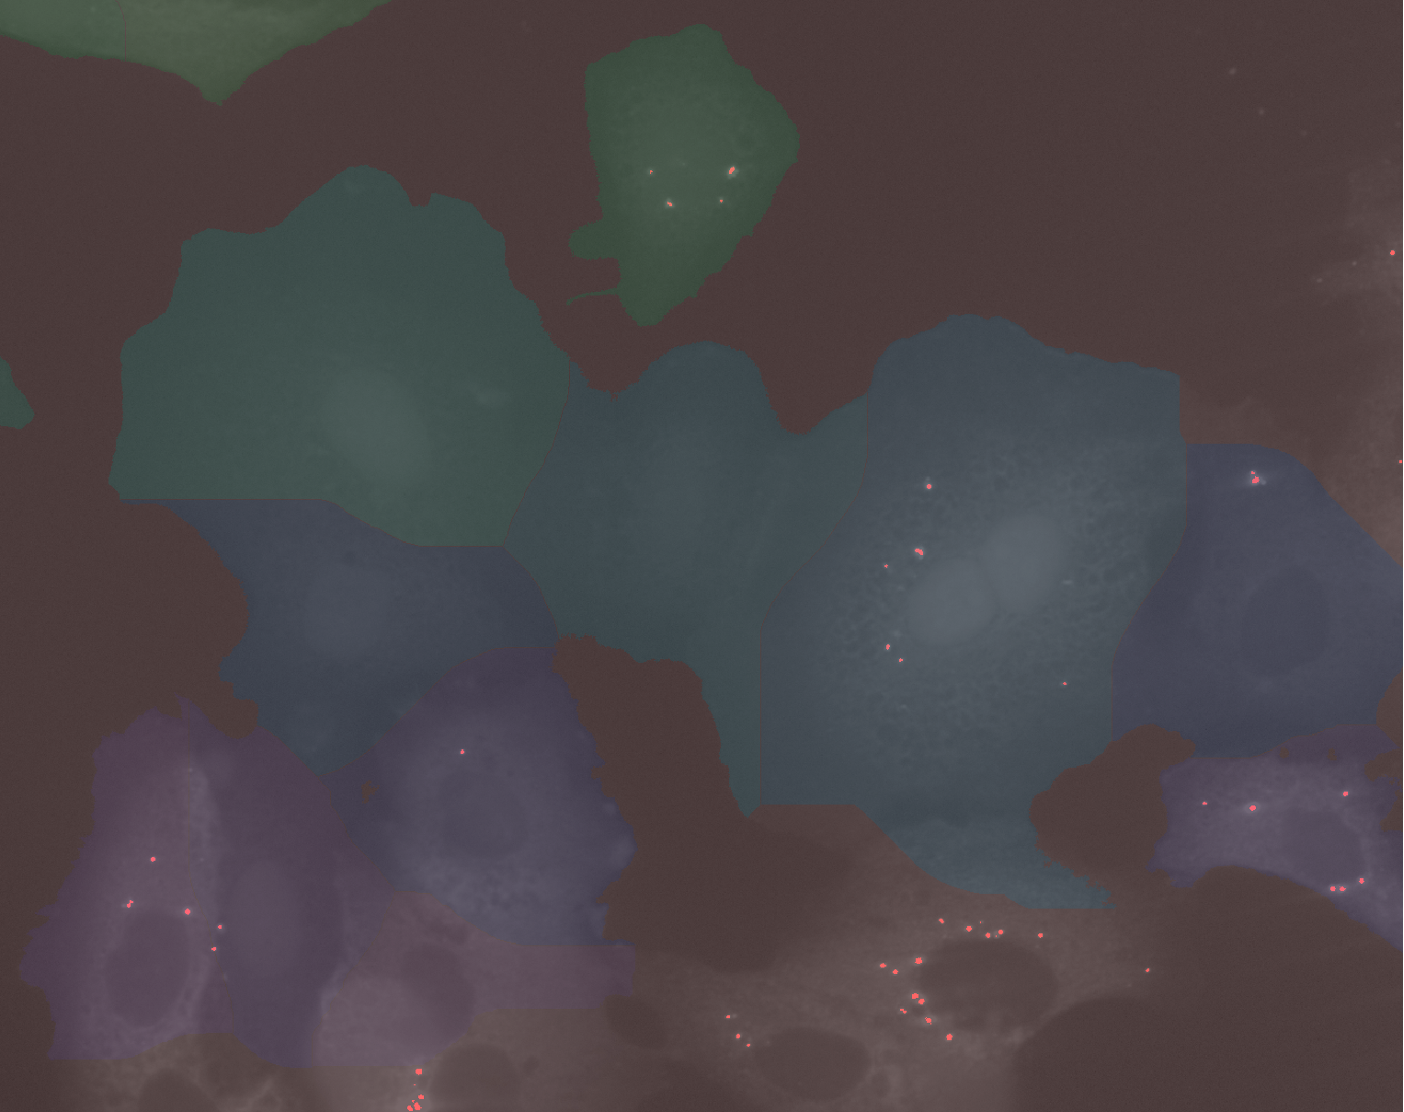
\includegraphics[width=0.9\textwidth]{overlayed.png}
            }
        }
    }\caption{Mask Overlapped with Predicted Labels}
    \label{fig:overlayed}
\end{figure}

Figure~\ref{fig:overlayed} shows the overlap of a filter on top of an image
with labeled condensates highlighted in red.

\subsection{Results}
\begin{figure}[H]
    \centering
    {
        {
            {
                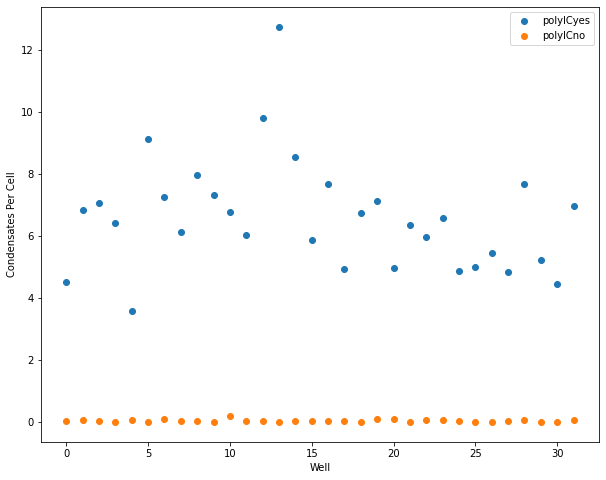
\includegraphics[width=0.7\textwidth]{well_results.png}
            }
        }
    }\caption{Counts of Wells of Different added Compounds}
    \label{fig:well_results}
\end{figure}

\end{document}